\documentclass[12pt]{beamer}
\usetheme{Madrid}
\usepackage[utf8]{inputenc}
\usepackage[portuguese]{babel}
\usepackage[T1]{fontenc}
\usepackage{amsmath}
\usepackage{booktabs}
\usepackage{amsfonts}
\usepackage{amssymb}
\usepackage{graphicx}
\usepackage{capt-of}
\usepackage{tabularx}
\setbeamertemplate{navigation symbols}{} 
\colorlet{beamer@blendedblue}{green!60!black}
\logo{
\includegraphics[scale=0.03]{./img/uea-new.png}}
\usepackage[backend=biber]{biblatex}
\addbibresource{references.bib}

%------------- CAPA ----------------

\title{BURI}
\subtitle{Sistema Embarcado de monitoramento da qualidade do ar em ambiente residencial}
\author{Adevan Neves Santos \\ Orientador: Prof. Jonathas Silva dos Santos}

\date{12 de dezembro de 2024}

\setbeamertemplate{footline}{%
  \leavevmode%
  \hbox{%
    \begin{beamercolorbox}[wd=.33\paperwidth,ht=2.5ex,dp=1ex,center,leftskip=3mm]{author in head/foot}%
      \usebeamerfont{author in head/foot}Adevan Neves Santos
    \end{beamercolorbox}%
    \begin{beamercolorbox}[wd=.34\paperwidth,ht=2.5ex,dp=1ex,center]{title in head/foot}%
      \usebeamerfont{title in head/foot}\insertframenumber/\inserttotalframenumber
    \end{beamercolorbox}%
    \begin{beamercolorbox}[wd=.33\paperwidth,ht=2.5ex,dp=1ex,center,rightskip=3mm]{date in head/foot}%
      \usebeamerfont{date in head/foot}BURI
    \end{beamercolorbox}%
  }%
  \vskip0pt%
}

%------------- CAPA ----------------

% As dicas de cada seção foram retiradas do vídeo: https://www.instagram.com/p/DCCn51VxLwa/

\begin{document}
    \maketitle

    \begin{frame}
        \frametitle{Sumário}
        \tableofcontents
    \end{frame}

    \section{Introdução}
    %Apresente o título do TCC e introduza rapidamente o contexto
    %pergunta de pesquisa e os objetivos

    \begin{frame}{Contextualização}
        O monóxido de carbono (CO) é uma substância química incolor, inodoro e asfixiante. Atua no organismo humano pelo processo 
        de transporte de oxigênio no sangue \cite{carbon-monoxide-poisoning-varon}.
        \begin{figure}[ht]
            \centering
            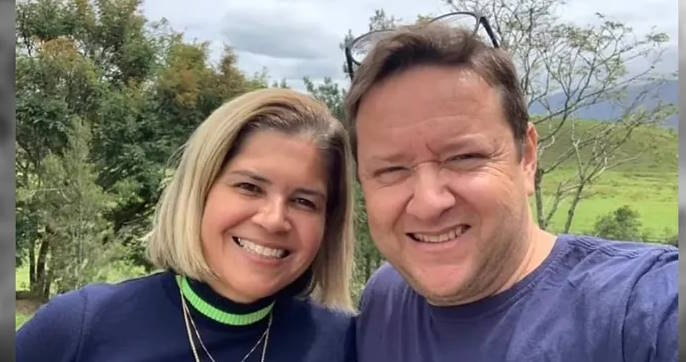
\includegraphics[width=0.55\textwidth]{img/morte-co.jpg}
            \caption{Apuração da perícia policial confirma morte por intoxicação de monóxido de carbono. Fonte: \cite{noticia-manaus-fumaca}}\label{fig:context}
        \end{figure}         
    \end{frame}

    \begin{frame}{Objetivo Geral}
        O objetivo geral é oferecer uma solução de sistema embarcado para o monitoramento
        da qualidade do ar em ambiente residencial, com ênfase na coleta de dados e identificação de
        condições de risco. 
    \end{frame}

    \begin{frame}{Objetivos Específicos}
        Portanto, para alcançar o objetivo geral, é necessário cumprir os seguintes objetivos específicos:
        \begin{itemize}
            \item Elaborar pesquisa com potenciais usuários e realizar avaliação do sistema;
            \item Coletar, compreender e tratar as informações dos sensores de: monóxido de carbono, temperatura e umidade do ar;
            \item Construir o protótipo do dispositivo embarcado;
            \item Realizar a comunicação entre o dispositivo e os demais módulos da aplicação;
            \item Desenvolver a API de dados e eventos, assim como a interface do sistema com o usuário;
        \end{itemize} 
    \end{frame}

    \section{Justificativa}
    %Explique a relevância do trabalho de forma sucinta, justificam
    %sua importância acadêmica ou prática.

    \begin{frame}{Justificativa}
        O monitoramento da concentração de monóxido de carbono, um gás tóxico e imperceptível, é decisivo para prevenir riscos 
        à saúde e garantir a segurança das pessoas em ambiente fechado, como o caso de residências. Ao automatizar a detecção e 
        emissão de alerta, o sistema proposto proporciona poder de decisão, contribuindo para a redução de acidentes
        relacionados a esse poluente em ambientes residenciais.   
    \end{frame}

    \section{Referencial Teórico}
    %Destaque os principais conceitos e autores que embasam o
    %trabalho, sem entrar em detalhes excessivos.

    \begin{frame}{Referencial Teórico}
        O desenvolvimento do protótipo abordou diversos temas, entre eles: 
        IoT, redes de computadores e estudo do monóxido de carbono. Além disso, o sistema 
        \textbf{BURI} utilizou trabalhos acadêmicos para embasar a fundamentação teórica. Portanto, 
        serão abordados a seguir, sucintamente, alguns tópicos importantes de cada área.
    \end{frame}

    \begin{frame}{IoT}
        IoT é a sigla em inglês para o termo \textit{Internet of Things} (Internet das Coisas). 
        A expressão possui muitas definições, porém o significado mais comum é dispositivos eletrônicos 
        conectados à rede mundial de computadores, recebendo e enviando dados.
        \begin{figure}[ht]
            \centering
            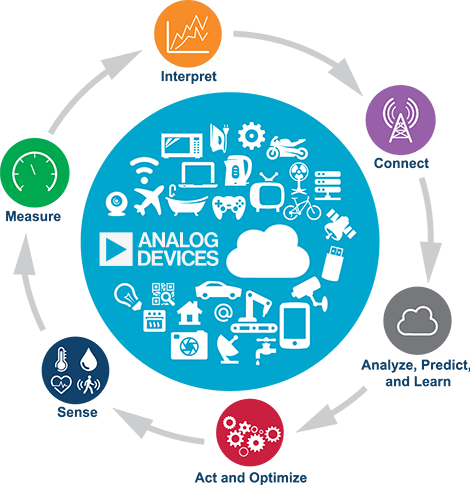
\includegraphics[width=0.38\textwidth]{img/iot-cycle.png}
            \caption{Ciclo do IoT. Fonte: \cite{iot-cycle}}\label{fig:cycleIoT}
        \end{figure}
    \end{frame}

    \begin{frame}{Redes de Computadores}
        ``A internet é um subsistema de comunicação único que fornece comunicação entre todos os hosts conectados a ela'' \cite[pp. 96]{sistemas-distribuidos-coulouris2013}. Dentro do 
        assunto de redes locais de conexão sem fio, existe dois representantes: Wi-Fi e Bluetooth. 
        
        Uma rede Wi-Fi permite conexão de alta velocidade entre \textit{hosts} ou hospedeiros via 
        pontos de acesso (\textit{access point} - AP). Já o protocolo Bluetooth é projetado para conexões de curto alcance e de baixa potência entre dois dispositivos.
    \end{frame}

    \begin{frame}{Monóxido de carbono}
        \begin{figure}[ht]
            \centering
            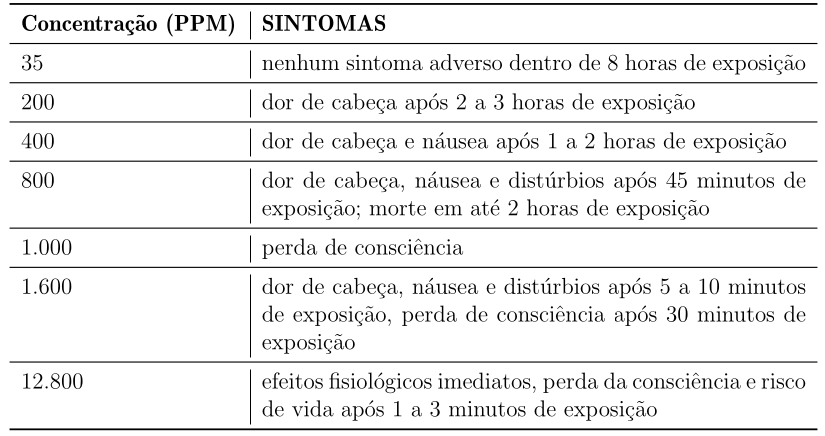
\includegraphics[width=0.88\textwidth]{img/tab-concentracao-co.png}
            \caption{Concentração de CO e efeitos. Fonte: \cite{seguranca-contra-incendios}}\label{fig:co}
        \end{figure}
    \end{frame}    

    \begin{frame}{Trabalhos Relacionados}
        \begin{enumerate}
            \item Desenvolvimento de um protótipo de dispositivo de baixo custo baseado em Iot (internet of things) para detecção e prevenção de incêndios em ambientes residenciais \cite{uea-iot-deteccao-incendio}.
            \item \textit{Indoor Air Quality Monitoring on AWS Using MQTT Protocol} \cite{iot-monitoring-on-aws}.
            \item AirWorld: uma solução tecnológica para o monitoramento da qualidade do ar em ambientes públicos \cite{UFAMAirWorld}.
            \item \textit{Intelligent based novel embedded system based IoT enabled
            air pollution monitoring system} \cite{tbRelacionado4NovelEmbeddedSystem}.
            \item Automação residencial de monitoramento de gás por meio da plataforma Arduino e IOT \cite{alexandre-automaccao-formulas-de-leitura-sensor}.
        \end{enumerate}
    \end{frame}

    \section{Metodologia}
    %Resuma a metodologia utilizada, incluindo o tipo de pesquisa,
    %métodos de coleta e análise de dados

    \begin{frame}{Metodologia}
        A metodologia do trabalho de conclusão de curso basea-se no \textit{embedded design lifecycle diagram} \cite{system-design-IOT}, diagrama de atividades 
        apresentado no livro \textit{Embedded Systems Design}, mas com adaptações para o contexto acadêmico.

        \begin{figure}[ht]
            \centering
            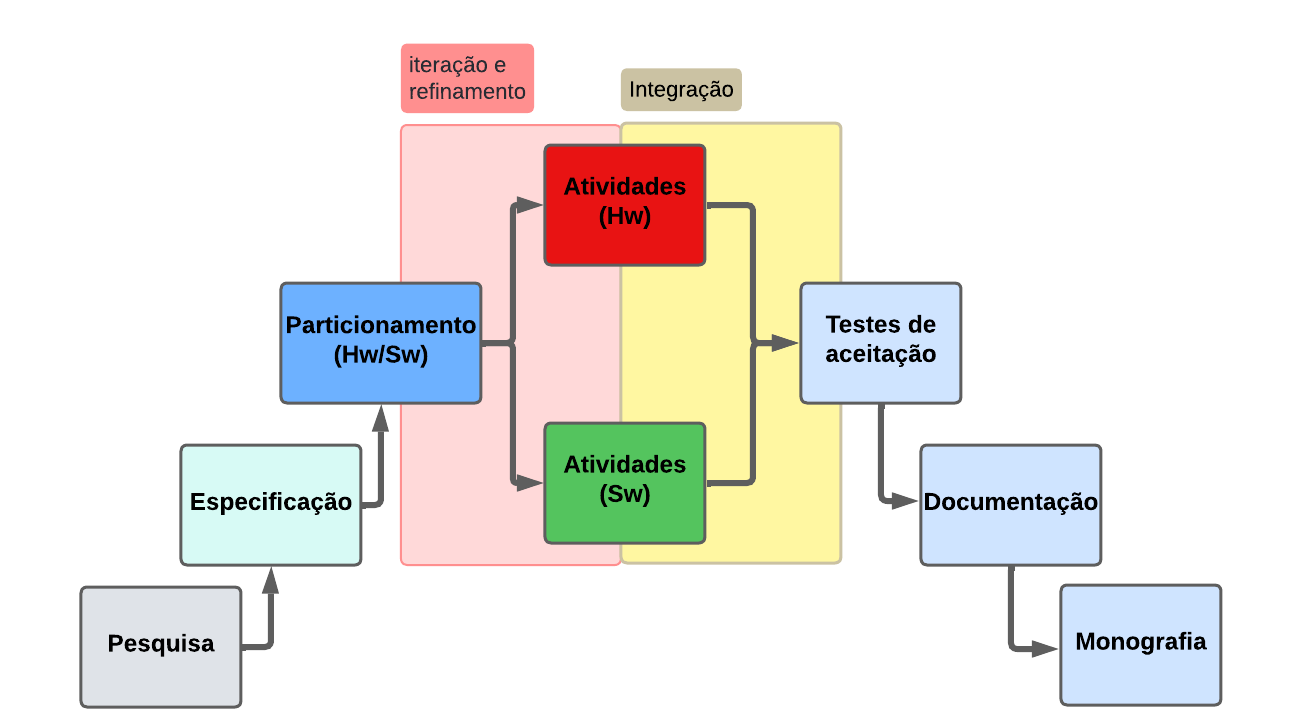
\includegraphics[width=0.74\textwidth]{img/diagrama-metodologia.png}
            \caption{Metodologia. Fonte: Autor, com base em \cite{system-design-IOT}}\label{fig:metodologia}
        \end{figure}
    \end{frame}

    \begin{frame}{Metodologia: Atividades Realizadas}
        \begin{figure}[ht]
            \centering
            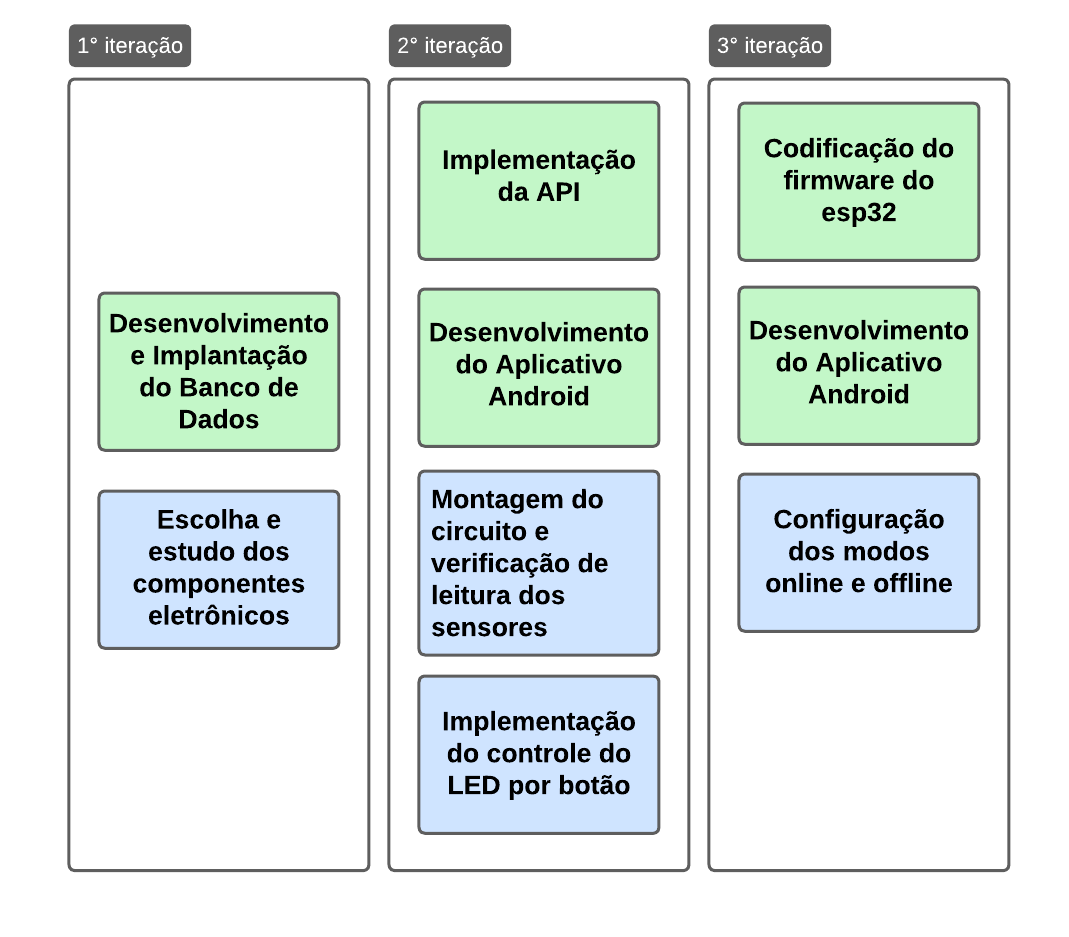
\includegraphics[width=0.66\textwidth]{img/tarefas-metodologia.png}
            \caption{Atividades de desenvolvimento. Fonte: Autor}\label{fig:atv}
        \end{figure}
    \end{frame}

    \section{Resultados}
    %Foque nos resultados mais relevantes e significativos,
    %destacando como eles respondem à pergunta de pesquisa.

    \begin{frame}{Resultados: Protótipo Físico}
        \begin{figure}[ht]
            \centering
            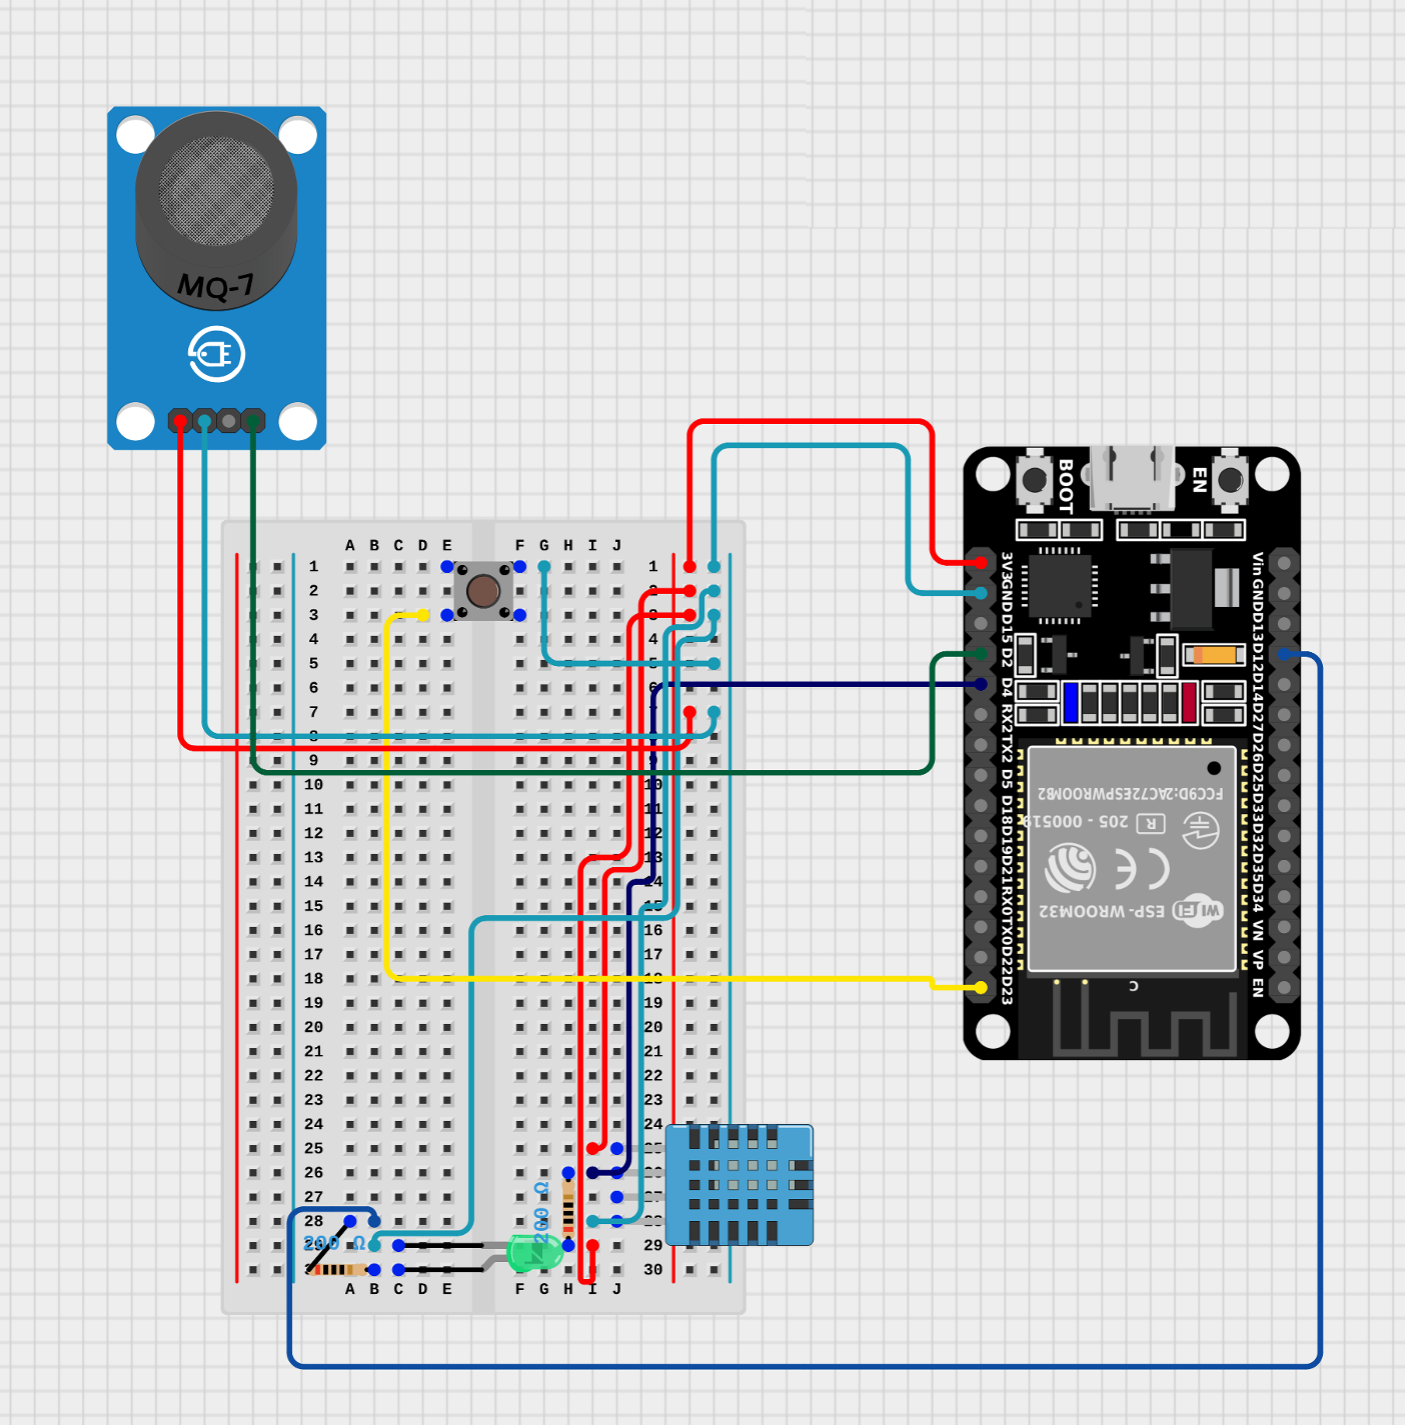
\includegraphics[width=0.57\textwidth]{img/buri-esquematico.png}
            \caption{Esquemático do \textit{hardware}. Fonte: Autor}\label{fig:hardware}
        \end{figure}
    \end{frame}

    \begin{frame}{Resultados: Aplicativo Android}
        \begin{figure}[ht]
            \centering
            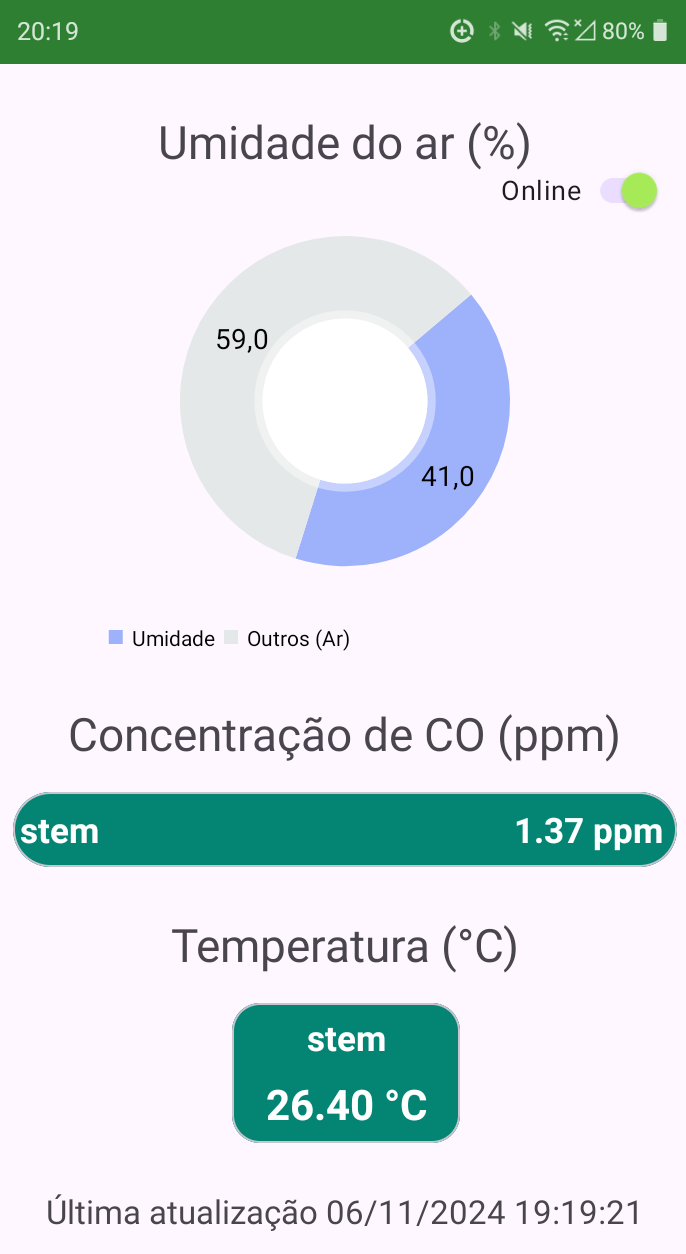
\includegraphics[width=0.27\textwidth]{img/app.png}
            \caption{Monitoramento pelo aplicativo. Fonte: Autor}\label{fig:software}
        \end{figure}
    \end{frame}

    \begin{frame}{Resultados: Notificação de alerta}
        O dispositivo embarcado lida com informação crítica. Conforme ilustrado na Figura \ref{fig:co}, 
        altas concentrações de CO combinadas com período curto de tempo são fatais. Portanto, o \textit{software} 
        implementa o aviso de exposição na forma de notificações do aplicativo e monitora cada medição para 
        determinar a criação de um novo evento no Banco de Dados.
    \end{frame}

    \begin{frame}{Resultados: Notificação de alerta}
        \begin{figure}[ht]
            \centering
            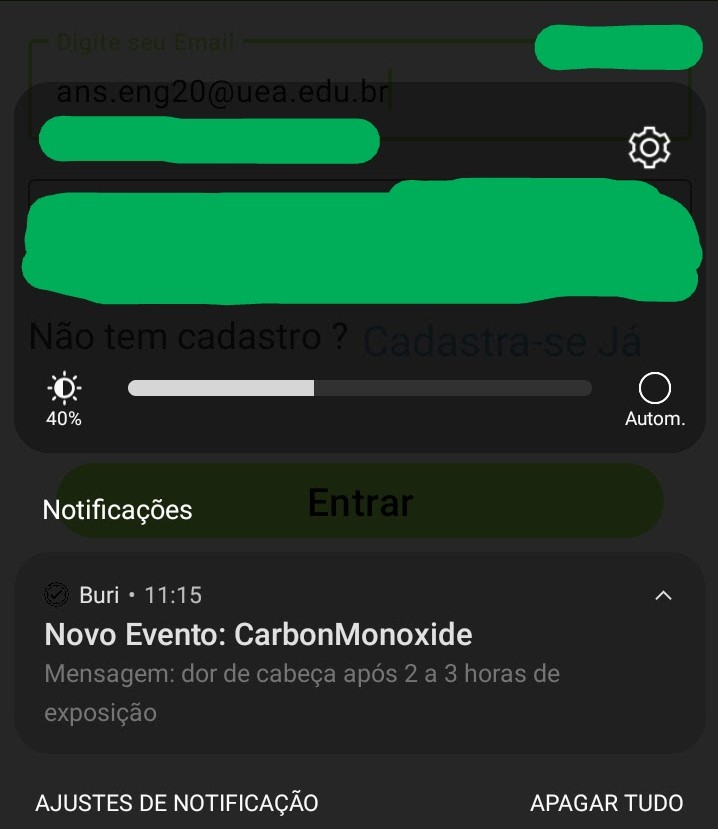
\includegraphics[width=0.47\textwidth]{img/notificação.jpg}
            \caption{Notificação no \textit{smartphone}. Fonte: Autor}\label{fig:notification}
        \end{figure}
    \end{frame}

    \begin{frame}{Resultados: Questionário e Teste de aceitação}
        Após a conclusão das atividades listadas na Figura \ref{fig:atv}, a próxima fase foi 
        a aplicação do teste de aceitação. Essa etapa consiste na criação de atividades práticas e escolha de um 
        grupo de pessoas para executarem ações no sistema. Portanto, o total de 38 alunos de graduação foram voluntários 
        para o processo mencionado anteriormente.
    \end{frame}

    \begin{frame}{Resultados: Questionário e Teste de aceitação}
        \begin{figure}[ht]
            \centering
            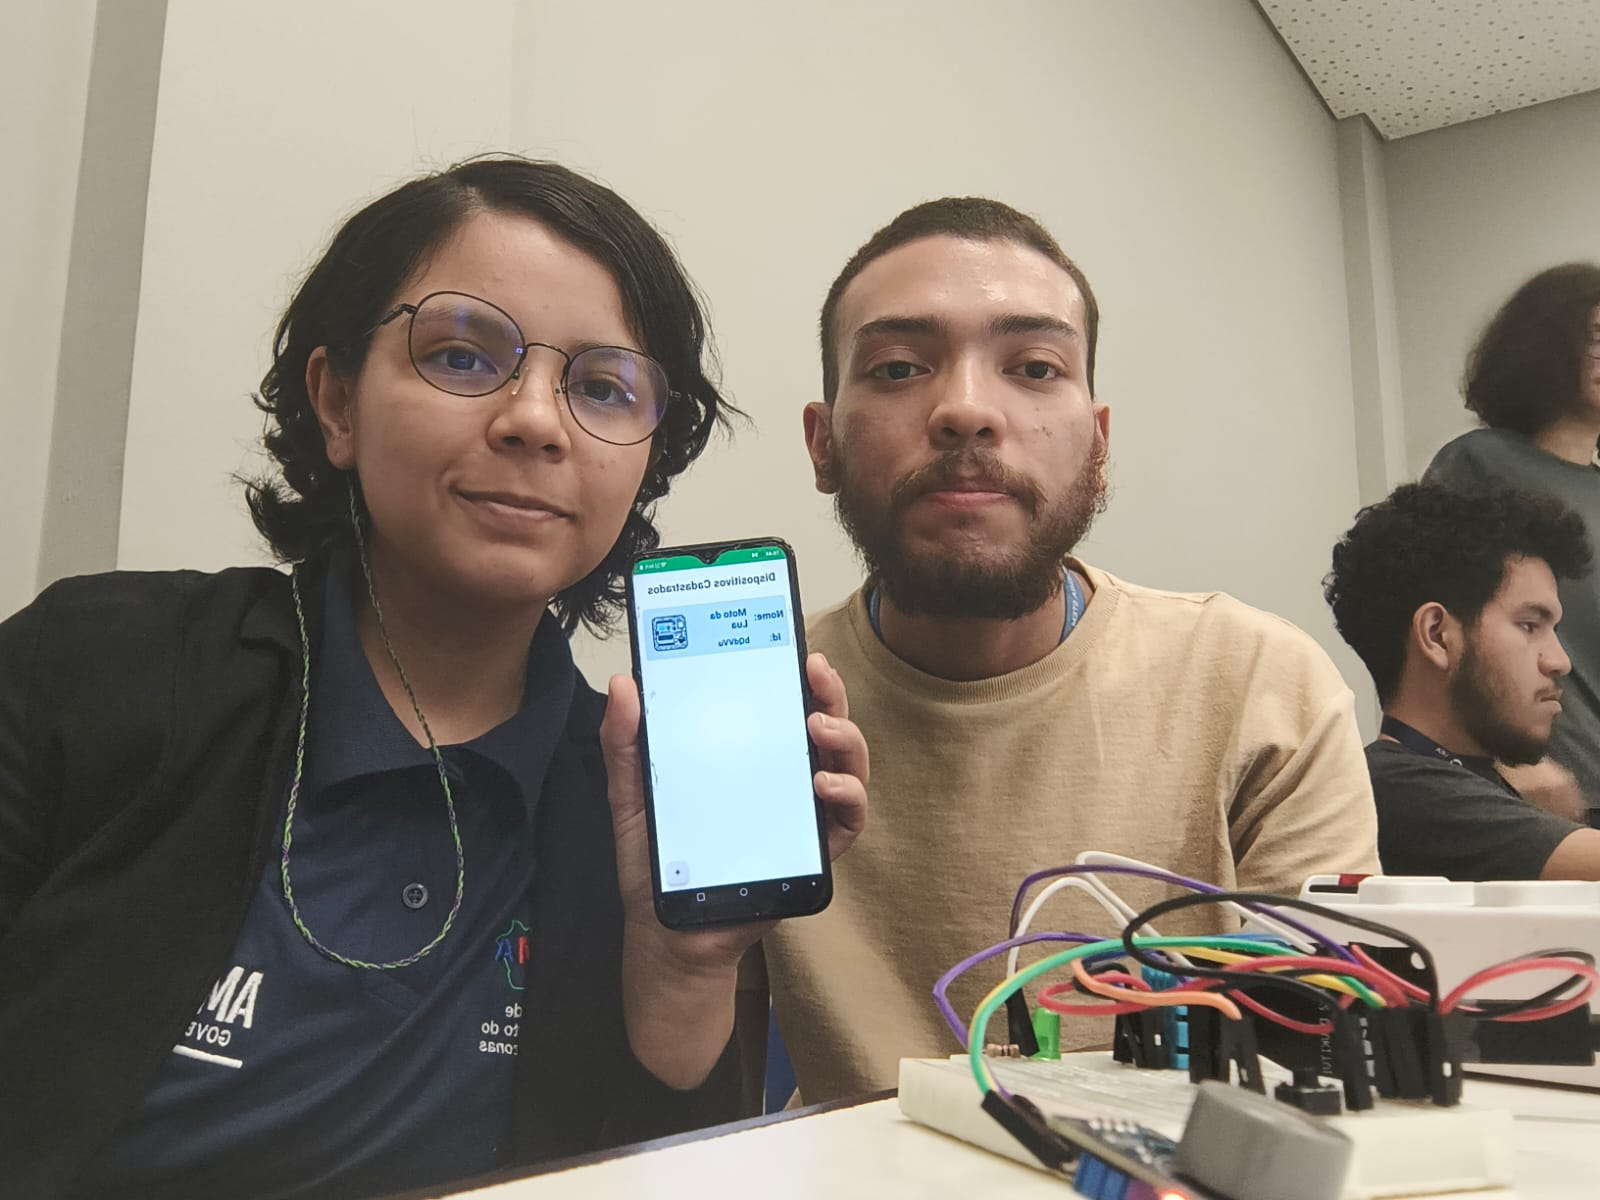
\includegraphics[width=0.40\textwidth]{img/teste/app1.jpeg}
            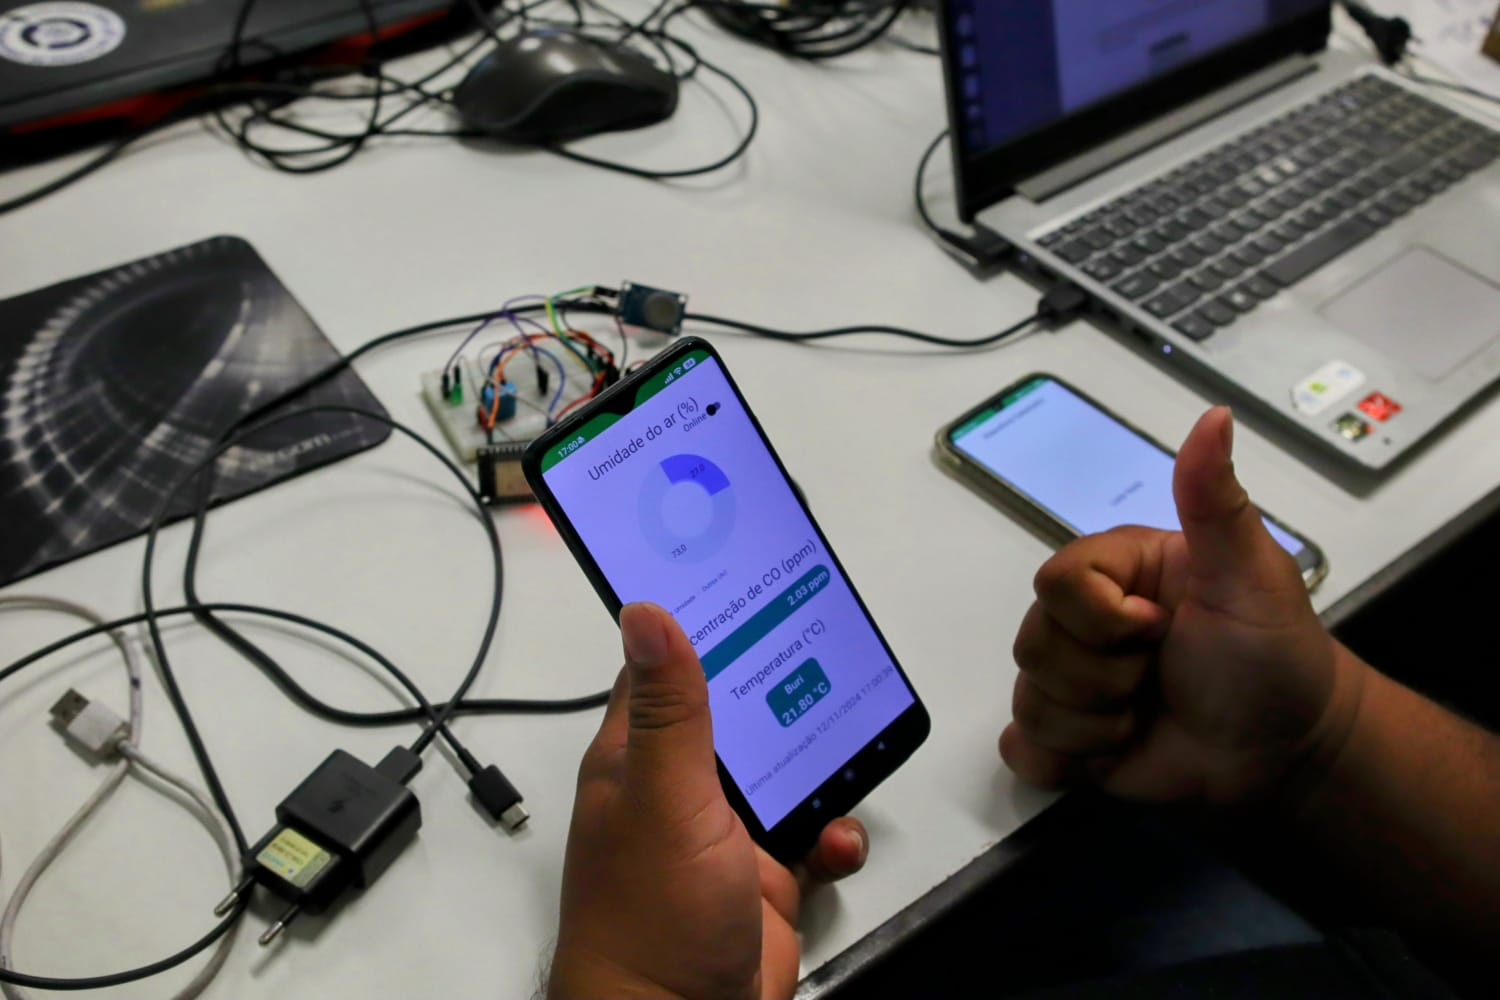
\includegraphics[width=0.45\textwidth]{img/teste/hard2.jpeg}
            \caption{Testes do sistema BURI. Fonte: Autor.}\label{fig:testes-fotos}
        \end{figure}
    \end{frame}

    \begin{frame}{Resultados: Questionário e Teste de aceitação}
        Durante a avaliação, os entrevistados realizaram 8 atividades:
        \begin{enumerate}
            \item Criar conta;
            \item Fazer Login;
            \item Cadastrar novo dispositivo;
            \item Visualizar lista de dispositivos cadastrados;
            \item Selecionar dispositivo;
            \item Visualizar dados (\textit{online});
            \item Visualizar dados (\textit{offline});
            \item Mudar propriedade de dispositivo;
        \end{enumerate}
    \end{frame}

    \section{Discussão}
    %Relacione os resultados com o referencial teórico e com outros
    %estudos, interpretando o que eles significam

    \begin{frame}{Discussão: Análise das respostas do questionário}
        O uso de questionário foi necessárias em duas etapas do projeto: especificação e testes 
        de aceitação. Na especificação, o objetivo é coletar dados sobre o ambiente da casa, percepção dos 
        alunos sobre o uso de um sistema de monitoramento e noção de custo para implantação do protótipo.
        Na segunda fase, o questionário busca obter dados sobre a experiência de uso do aplicativo.
    \end{frame}

    \begin{frame}{Discussão: Primeiro questionário}   
        Custo total do \textit{hardware}: R\$ 146,25
        
        \begin{figure}[ht]
            \centering
            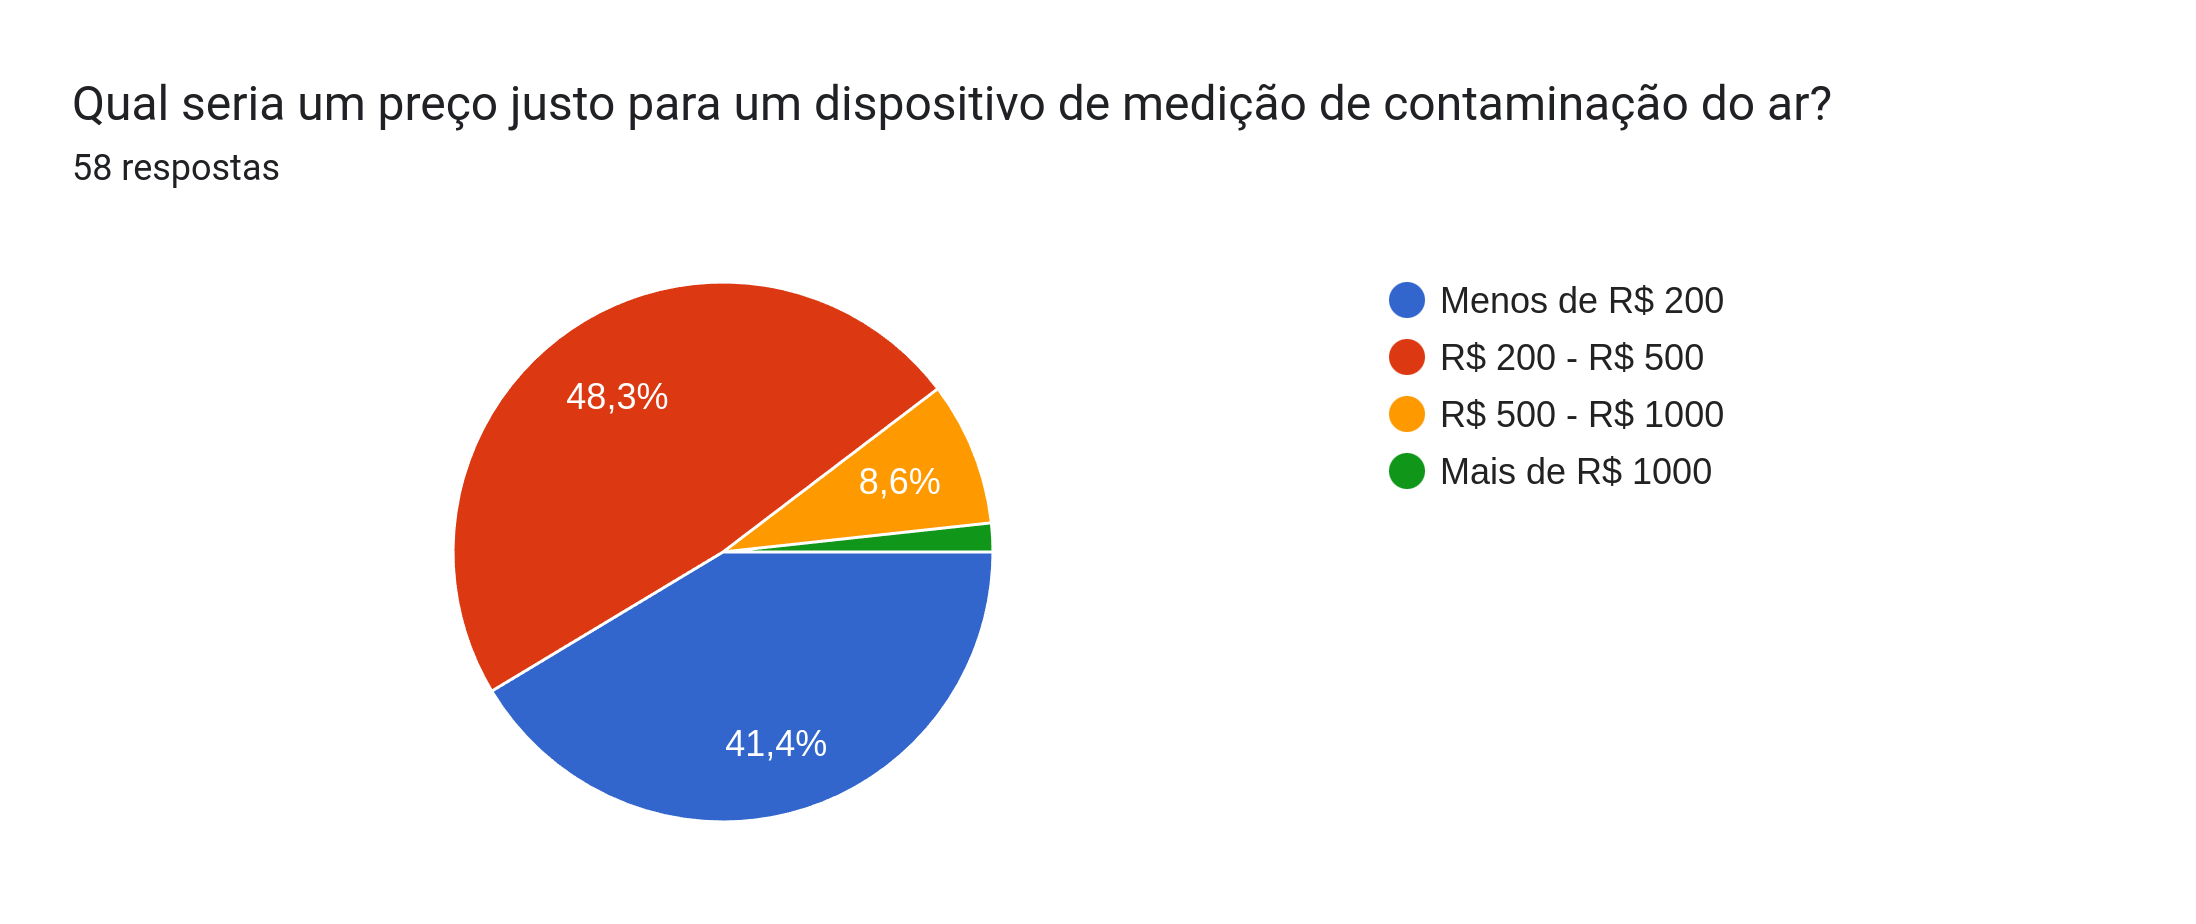
\includegraphics[width=0.99\textwidth]{./img/grafico-preco-hardware.png}
            \caption{Preço justo. Fonte: Autor}\label{fig:precoJusto}
        \end{figure}
    \end{frame}

    \begin{frame}{Discussão: Primeiro questionário}        
        \begin{figure}[ht]
            \centering
            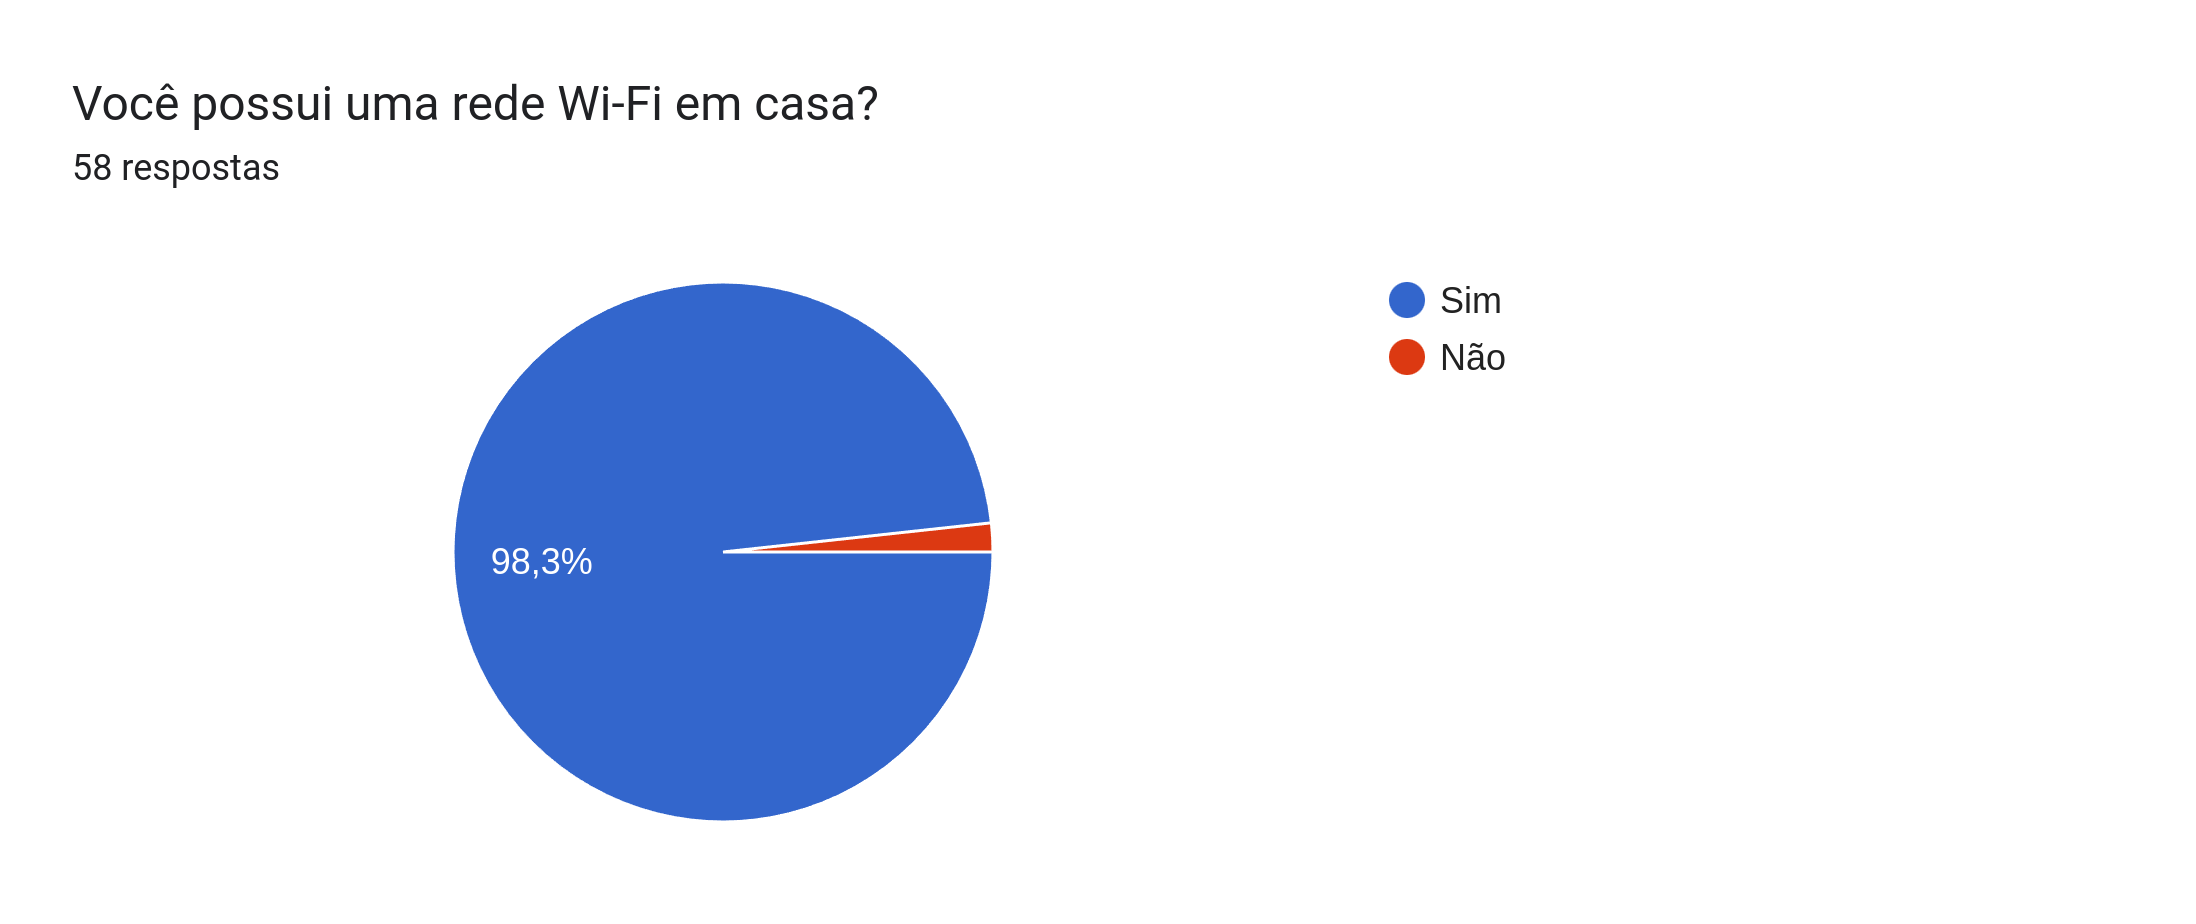
\includegraphics[width=0.99\textwidth]{./img/questionario-wifi.png}
            \caption{Pergunta sobre Wi-Fi. Fonte: Autor}\label{fig:wifi}
        \end{figure}
    \end{frame}

    \begin{frame}{Discussão: Segundo questionário}
        \begin{figure}[ht]
            \centering
            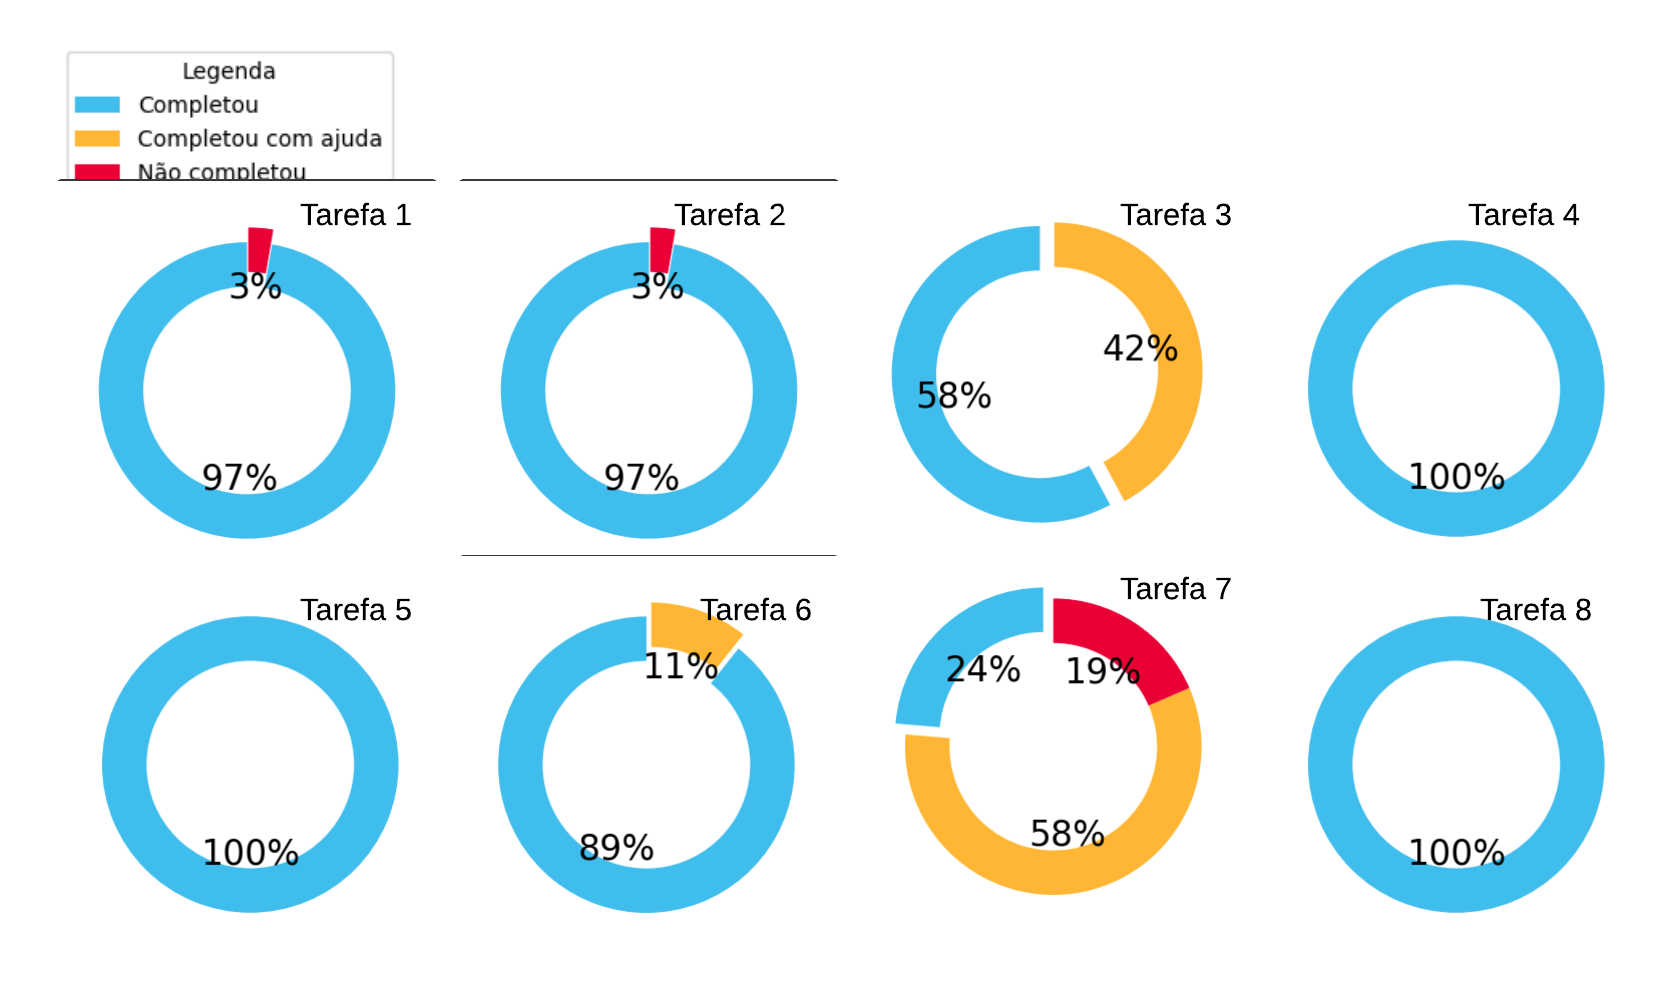
\includegraphics[width=0.90\textwidth]{./img/grafico-tarefas-teste-buri.png}
            \caption{Desempenho dos alunos. Fonte: Autor}\label{fig:atvBuri}
        \end{figure}
    \end{frame}

    \begin{frame}{Discussão: Segundo questionário}
        \begin{figure}[ht]
            \centering
            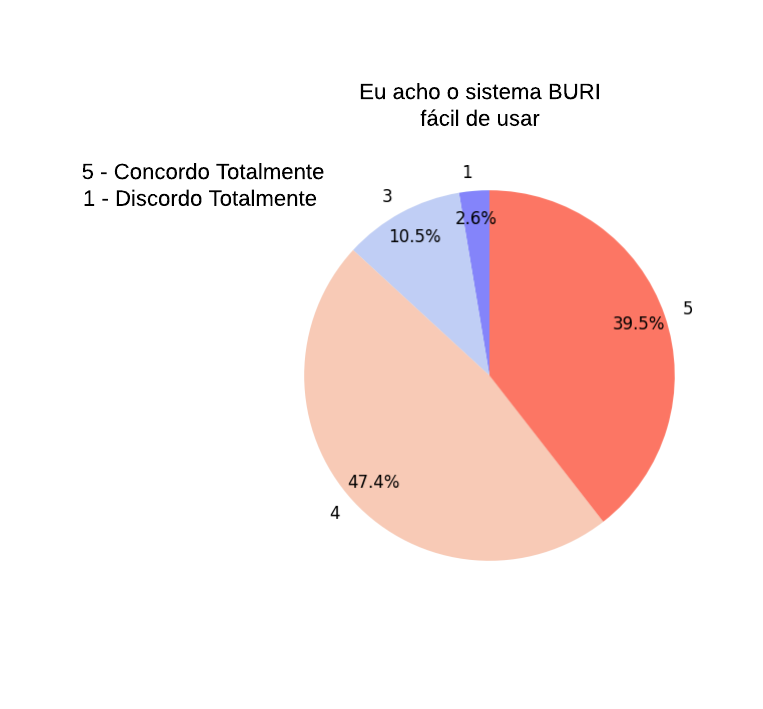
\includegraphics[width=0.60\textwidth]{./img/grafico-sistema-eh-facil-usar.png}
            \caption{Facilidade do sistema. Fonte: Autor}\label{fig:buriFacilDeUsar}
        \end{figure}
    \end{frame}

    \begin{frame}{Discussão: Comparação com trabalhos relacionados}
        \begin{figure}[ht]
            \centering
            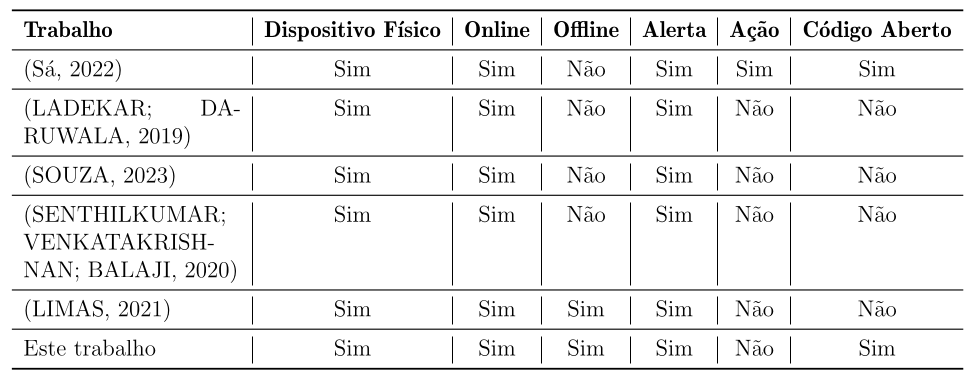
\includegraphics[width=0.90\textwidth]{./img/comparacao-trabalho.png}
            \caption{Trabalhos de referência e o Buri. Fonte: Autor}\label{fig:buriTRab}
        \end{figure}
    \end{frame}

    \section{Considerações Finais}
    %Enfatize as conclusões e implicações principais, 
    %incluindo sugestões para pesquisas futuras.

    \begin{frame}{Considerações Finais}
        O sistema BURI é uma proposta de solução para o monitoramento da qualidade do
        ar em residências, com possibilidade de aplicação em outros ambientes \textit{indoor}. Seu objetivo é
        operar de forma integrada com o \textit{smartphone} do usuário e a rede Wi-Fi, embora o módulo de
        monitoramento também ofereça comunicação offline por meio de Bluetooth. 
    \end{frame}

    \begin{frame}{Trabalhos Futuros}
        \begin{enumerate}
            \item Implantação do servidor na nuvem;
            \item Identificar e corrigir mau comportamento na conexão Bluetooth;
            \item Melhorar a interface de pop-up na ação de ``COPIAR URL'';
            \item Testar outras abordagens de configuração do protótipo além da biblioteca \textit{Wifi Manager};
        \end{enumerate}
    \end{frame}

    \section{Referências}

    \begin{frame}{Referências}
    
    \end{frame}
    
    \printbibliography
\end{document}